\documentclass{standalone}
\usepackage{pgfplots}
\usepackage{pgfplotstable}
\usepgfplotslibrary{fillbetween}
\usetikzlibrary{arrows.meta, positioning, backgrounds}

\begin{document}

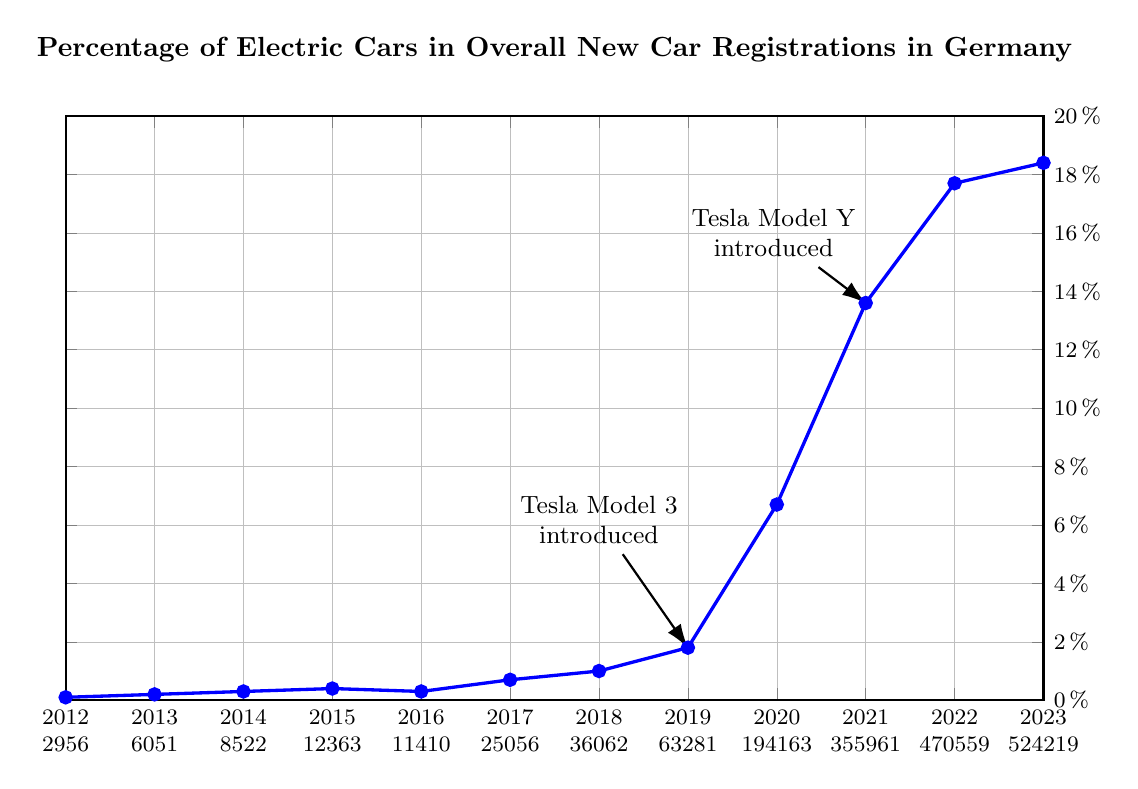
\begin{tikzpicture}
    \begin{axis}[
        title={Percentage of Electric Cars in Overall New Car Registrations in Germany},
        width=14cm,
        height=9cm,
        xmin=2012, xmax=2023,
        ymin=0, ymax=20,
        xtick={2012,2013,2014,2015,2016,2017,2018,2019,2020,2021,2022,2023},
        ytick={0,2,4,6,8,10,12,14,16,18,20},
        xticklabels={2012\\2956,2013\\6051,2014\\8522,2015\\12363,2016\\11410,2017\\25056,2018\\36062,2019\\63281,2020\\194163,2021\\355961,2022\\470559,2023\\524219},
        xticklabel style={/pgf/number format/1000 sep=},
        xticklabel style={rotate=0, anchor=north, align=center},
        yticklabel pos=right,
        yticklabel={
            \pgfmathprintnumber{\tick}\,\%
        },
        grid=both,
        major grid style={line width=.2pt,draw=gray!50},
        minor grid style={line width=.1pt,draw=gray!20},
        thick,
        every axis plot/.append style={thick},
        every mark/.append style={scale=1.2},
        legend style={draw=none, at={(0.95,0.05)}, anchor=south east, fill=none, font=\small},
        title style={font=\bfseries, align=center, yshift=10pt},
        tick label style={font=\footnotesize},
    ]
    \addplot[
        color=blue,
        mark=*,
        mark options={fill=blue},
        line width=1.2pt
    ] coordinates {
        (2012, 0.1)
        (2013, 0.2)
        (2014, 0.3)
        (2015, 0.4)
        (2016, 0.3)
        (2017, 0.7)
        (2018, 1.0)
        (2019, 1.8)
        (2020, 6.7)
        (2021, 13.6)
        (2022, 17.7)
        (2023, 18.4)
    };

    % Add annotation for Tesla Model 3
    \node[fill=none, text=black, align=center, font=\small, anchor=south east] (model3) at (axis cs:2019,5) {Tesla Model 3\\introduced};
    \draw[{Latex[length=3mm, width=2mm]}-, thick] (axis cs:2019,1.8) -- (model3);

    % Add annotation for Tesla Model Y
    \node[fill=none, text=black, align=center, font=\small, anchor=east] (modely) at (axis cs:2021,16) {Tesla Model Y\\introduced};
    \draw[{Latex[length=3mm, width=2mm]}-, thick] (axis cs:2021,13.6) -- (modely);

    \end{axis}
\end{tikzpicture}

\end{document}